\section{矩阵相似与可对角化}

矩阵相似是指两个矩阵可以通过相似变换互相转换, 而矩阵可对角化是指将一个矩阵通过相似变换变为对角矩阵。两者之间的关系是:如果一个矩阵可对角化, 则它必定与某个对角矩阵相似;反之, 如果两个矩阵相似, 则它们可能都可对角化, 但不一定其中之一必定可对角化.

\subsection{矩阵的相似}

\begin{definition}[矩阵的相似]
    设 $\vb*{A}\text{, }\vb*{B}$ 是 $n$ 阶矩阵, 如果存在 $n$ 阶可逆矩阵 $\vb*{P}$, 使得 $$\vb*{P}^{-1}\vb*{AP}=\vb*{B}$$
    \index{矩阵相似}则称矩阵 $\vb*{A}$ 与 $\vb*{B}$ \textit{相似}, 记为 $\vb*{A}\sim\vb*{B}.$
\end{definition}

\begin{theorem}[相似的反身性]
    任意矩阵都与其自身相似, 即对于任意矩阵 $\vb*{A}$, 存在一个非奇异矩阵 $\vb*{E}$ (单位矩阵), 使得:
    $$\vb*{A}=\vb*{E}^{-1} \vb*{A I}=\vb*{A}.$$
\end{theorem}

\begin{theorem}[相似的对称性]
    如果矩阵 $\vb*{A}$ 和 $\vb*{B}$ 相似, 即存在一个非奇异矩阵 $\vb*{T}$ 使得:
    $$\vb*{B}=\vb*{T}^{-1} \vb*{A T}$$
    那么 $\vb*{A}$ 和 $\vb*{B}$ 也相似, 即存在一个非奇异矩阵 $\vb*{S}$ 使得:
    $$\vb*{A}=\vb*{S}^{-1} \vb*{B S}.$$
\end{theorem}

\begin{theorem}[相似的传递性]
    如果矩阵 $\vb*{A}$ 和 $\vb*{B}$ 相似, 且 $\vb*{B}$ 和 $\vb*{C}$ 相似, 那么 $\vb*{A}$ 和 $\vb*{C}$ 也相似, 即存在非奇异矩阵 $\vb*{T}$ 和 $\vb*{S}$ 使得:
    $$\vb*{B}=\vb*{T}^{-1} \vb*{A T}, \quad \vb*{C}=\vb*{S}^{-1} \vb*{B S}$$
    则存在一个非奇异矩阵 $\vb*{U}$ 使得:
    $$\vb*{A}=\vb*{U}^{-1} \vb*{C U}.$$
\end{theorem}

\begin{theorem}[矩阵相似的必要条件]
    若 $\vb*{A}$ 与 $\vb*{B}$ 是相似的, 则由相似矩阵的性质可得:
    \setcounter{magicrownumbers}{0}
    \begin{table}[H]
        \centering
        \caption{矩阵相似的必要条件}
        \begin{tabular}{l l l l}
            (\rownumber) $\det\vb*{A}=\det\vb*{B}.$      & (\rownumber) $\rank(\vb*{A})=\rank\vb*{B}.$ & (\rownumber) $\tr\vb*{A}=\tr\vb*{B}.$        & (\rownumber) $|\lambda\vb*{E}-\vb*{A}|=|\lambda\vb*{E}-\vb*{B}|.$ \\
            \midrule
            (\rownumber) $k\vb*{A}\sim k\vb*{B}$.        & (\rownumber) $\vb*{A}^{m}\sim\vb*{B}^{m}$.  & (\rownumber) $f(\vb*{A})\sim f(\vb*{B})$     & (\rownumber) $\vb*{AB}\sim \vb*{BA}.$                             \\
            \midrule
            (\rownumber) $\vb*{A}^{-1}\sim\vb*{B}^{-1}$. & (\rownumber) $\vb*{A}^*\sim\vb*{B}^*.$      & (\rownumber) $\vb*{A}^\top\sim\vb*{B}^\top$.
        \end{tabular}
    \end{table}
\end{theorem}

\begin{example}
    已知矩阵 $\vb*{A}\sim\vb*{B}$, 其中 $\vb*{B}=\mqty(0&0&1\\0&2&0\\3&0&0)$, 则 $|\vb*{A}+\vb*{E}|$.
\end{example}
\begin{solution}
    因为 $\vb*{A}\sim\vb*{B}$, 则 $|\vb*{A}+\vb*{E}|=|\vb*{B}+\vb*{E}|=-6.$
\end{solution}

\begin{example}
    已知矩阵 $\vb*{A}=\mqty(-2& -2& 1\\ 2& x& -2\\ 0& 0& -2)$ 与 $\vb*{B}=\mqty(2& 1& 0\\ 0& -1& 0\\ 0& 0& y)$ 相似, 求 $x$ 与 $y$.
\end{example}
\begin{solution}
    因为 $\vb*{A}$ 与 $\vb*{B}$ 相似, 故具有相同的迹和相同的行列式, 故 $\left\{\begin{matrix}
            x-4=1+y \\
            4x-8=-2y
        \end{matrix}\right.\Rightarrow x=3\text{, }y=-2.$
\end{solution}

\begin{example}
    设 $\vb*{A}=\mqty(1&0&0\\0&1&0\\2&2&-3)~,\vb*{B}=\mqty(1&2&0\\0&1&4\\0&0&-3)~,\vb*{C}=\mqty(2&1&-5\\0&1&0\\1&1&-4)~,\vb*{D}=\mqty(2&3&4\\0&1&-2\\5&1&-2)~,\vb*{\Lambda}=\diag(1,1,-3)$, 则在 $\vb*{A},\vb*{B},\vb*{C},\vb*{D}$ 中与 $\vb*{\Lambda}$ 相似的矩阵有
    \begin{tasks}(4)
        \task $\vb*{A},\vb*{C}$
        \task $\vb*{A},\vb*{D}$
        \task $\vb*{B},\vb*{C}$
        \task $\vb*{A},\vb*{D}$
    \end{tasks}
\end{example}
\begin{solution}
    矩阵相似有四个必要条件, 分别为: 秩相等, 迹相等, 行列式相等和特征多项式相等, 于是对于矩阵 $\vb*{D}$ 因为 $\tr\vb*{D}\neq\tr\vb*{\Lambda}$, 故排除选项 B、D, 又因为
    矩阵相似对角矩阵等价于它的每一个特征值的重数与其对应的线性无关的特征向量个数相等, 对于矩阵 $\vb*{B}$, 它的特征值显然是 $1,1,-3$ 与 $\vb*{\Lambda}$ 相同, 但是对于 $\lambda=1$ (二重),
    $$n-\rank(\lambda\vb*{E}-\vb*{B})=3-2=1\neq 2 (\text{特征值重数})$$
    因此矩阵 $\vb*{B}$ 关于特征值 1 仅一个线性无关的特征向量, 矩阵 $\vb*{B}$ 不能相似对角化为 $\vb*{\Lambda}$, 排除选项 C, 故选 A.
\end{solution}

\begin{example}[2013 数一]
    矩阵 $\vb*{A}=\mqty(1&a&1\\a&b&a\\1&a&1)$ 与 $\vb*{B}=\mqty(2&0&0\\0&b&0\\0&0&0)$ 相似的充要条件为
    \begin{tasks}(4)
        \task $a=0,b=2$
        \task $a=0,b$ 为任意常数
        \task $a=0,b=0$
        \task $a=2,b$ 为任意常数
    \end{tasks}
\end{example}
\begin{solution}
    因为矩阵 $\vb*{A}$ 是实对称矩阵, 矩阵 $\vb*{B}$ 是对角矩阵, 则 $\vb*{A}$ 与 $\vb*{B}$ 相似的充要条件是 $\vb*{A}$ 的特征值为 $2,b,0$,
    因为 $2$ 是 $\vb*{A}$ 的特征值, 那么 $$|2\vb*{E}-\vb*{A}|=0\Rightarrow a=0$$
    当 $a=0$ 时, $|\lambda\vb*{E}-\vb*{A}|=\lambda(\lambda-2)(\lambda-b)$
    那么 $\vb*{A}$ 的特征值为 $2,b,0$, 所以 $b$ 为任意常数即可, 选 B.
\end{solution}

\begin{example}[2009 兰州大学]
    已知矩阵 $\vb*{A}=\mqty(1&2&2\\2&a&2\\2&2&1)\text{, }\vb*{B}=\mqty(-1&0&0\\0&-1&0\\0&0&b)$, 问 $a\text{, }b$ 取何值时 $\vb*{A}$ 与 $\vb*{B}$ 相似? 并求可逆矩阵 $\vb*{P}$ 使得 $\vb*{P}^{-1}\vb*{AP}=\vb*{B}.$
\end{example}
\begin{solution}
    \textbf{法一: }由于 $\vb*{A}$ 与 $\vb*{B}$ 相似, 则它们的特征多项式相同, 所以 $|\lambda\vb*{E}-\vb*{A}|=|\lambda\vb*{E}-\vb*{B}|$, 即
    $$\mqty|\lambda-1 &-2 &-2\\-2 &\lambda-a &-2\\-2 &-2 &\lambda-1|=\mqty|\lambda+1 &0 &0\\0 &\lambda+1 &0\\0 &0 &\lambda-b|$$
    得 $(\lambda+1)\qty(\lambda^2-(3+a)\lambda+3a-8)=(\lambda+1)^2(\lambda-b)$, 比较两边的系数, 得 $a=1\text{, }b=5$, 那么
    $$f(\lambda)=\mqty|\lambda-1 &-2 &-2\\-2 &\lambda-1 &-2\\-2 &-2 &\lambda-1|\xlongequal[r_1-r_3]{r_2-r_3}(\lambda+1)^2\mqty|1 &0 &-1\\0 &1 &-1\\-2 &-2 &\lambda-1|=(\lambda+1)^2(\lambda-5)$$
    那么 $\vb*{A}$ 的特征值为 $-1$ (二重) 和 5, 则对应的特征向量依次为
    $$\vb*{\xi}_1=(-1,-1,0)^{\top}\text{, }\vb*{\xi}_2=(-1,0,-1)^{\top}\text{, }\vb*{\xi}_3=(1,1,1)^{\top}$$
    从而可得可逆矩阵 $\vb*{P}=(\vb*{\xi}_1,\vb*{\xi}_2,\vb*{\xi}_3)=\mqty(-1 &-1 &1\\1 &0 &1\\0 &1 &1)$, 容易验证有 $\vb*{P}^{-1}\vb*{AP}=\vb*{B}$, 故 $\vb*{P}$ 即使所求.\\
    \textbf{法二: }因为 $\vb*{A}$ 与 $\vb*{B}$ 相似, 所以具有相同的迹和相同的行列式, 即 $\tr\vb*{A}=\tr\vb*{B}\text{, }\det \vb*{A}=\det\vb*{B}$, 故
    $$2+a=-2+b\text{, }-3a+8=b$$ 解得 $a=1\text{, }b=5.$
\end{solution}

% \begin{example}
%     设 3 阶方阵 $\vb*{A}$ 和 $\vb*{B}$, 其中 $\vb*{A}=\mqty(1&2&3\\0&1&2\\0&0&1)\text{, }\vb*{B}=\mqty(1&0&0\\0&1&2\\0&0&1)$, 问: 矩阵 $\vb*{A}$ 与 $\vb*{B}$ 是否相似, 并说明理由.
% \end{example}
% \subsection{Hamilton-Cayley 定理}
% 
% \begin{example}
%     设 $\vb*{A}=\mqty(2&1&0\\0&2&1\\0&0&2)\text{, }f(x)=1+x+x^2+x^3+x^4+x^5+x^6+x^7$, 求 $f(\vb*{A}).$
% \end{example}
% \begin{solution}
%     易知 $\vb*{A}$ 的特征多项式 $g(\lambda)=(\lambda-2)^3$, 对 $f(\lambda)$ 利用带余除法, 得 $$f(\lambda)=g(\lambda)h(\lambda)+a\lambda^2+b\lambda+c$$
%     从而有 $$$$
% \end{solution}

\subsection{相似对角化}

\subsubsection{可相似对角化}

\begin{theorem}
    实对称矩阵一定能相似对角化.
\end{theorem}

\begin{theorem}
    若存在不相等的实数 $a,~b$, 使得 $(\vb*{A}-a\vb*{E})(\vb*{A}-b\vb*{E})=\vb*{O}$, 则矩阵 $\vb*{A}$ 一定能相似对角化.
\end{theorem}
\begin{proof}[{\songti \textbf{证}}]
    因为 $(\vb*{A}-a\vb*{E})(\vb*{A}-b\vb*{E})=\vb*{O}$, 所以 $$n=\rank((b-a)\vb*{E})=\rank[(\vb*{A}-a\vb*{E})-(\vb*{A}-b\vb*{E})]\leqslant \rank(\vb*{A}-a\vb*{E})+\rank(\vb*{A}-b\vb*{E})\leqslant n$$
    故 $\rank(\vb*{A}-a\vb*{E})+\rank(\vb*{A}-b\vb*{E})=n$, 因此 $\vb*{A}$ 的属于特征值 $a$ 的特征向量个数有 $n-\rank(\vb*{A}-a\vb*{E})$; 属于特征值 $b$ 的特征向量个数有 $n-\rank(\vb*{A}-b\vb*{E})$, 共有
    $$2n-\qty[\rank(\vb*{A}-a\vb*{E})+\rank(\vb*{A}-b\vb*{E})]=n$$
    又因为 $\vb*{A}$ 有 $n$ 个线性无关的特征向量等价于 $\vb*{A}$ 一定能相似对角化.
\end{proof}

\begin{example}
    设矩阵 $\vb*{A}=\begin{pmatrix} 0 & 2 & 0 \\ 1 & -1 & a+1 \\ 0 & 0 & 1 \\\end{pmatrix}, \vb*{B}=\begin{pmatrix} 1 & 0 & 0 \\ 0 & 1 & 0 \\ 0 & 0 & b \\\end{pmatrix}$, 且 $\vb*{A}$ 与 $\vb*{B}$ 相似, 求 $a+b.$
\end{example}
\begin{solution}
    因为 $\vb*{A}\sim \vb*{B}$, 所以 $\tr\vb*{A}=\tr\vb*{B}\Rightarrow b=-2$, 又 $\vb*{B}$ 为对角矩阵, 所以 $\vb*{A}$ 可相似对角化, 所以 $\rank(\vb*{E}-\vb*{A})=1$, 即
    $$
        \vb*{E}-\vb*{A}=\begin{pmatrix} 1 & -2 & 0 \\ -1 & 2 & -a-1 \\ 0 & 0 & 0 \\\end{pmatrix}\to \begin{pmatrix} 1 & -2 & 0 \\ 0 & 0 & -a-1 \\ 0 & 0 & 0 \\\end{pmatrix}
    $$
    因此 $a=-1$, 所以 $a+b=-3.$
\end{solution}

\begin{example}[2017 数一]
    已知矩阵 $\vb*{A}=\mqty(2&0&0\\0&2&1\\0&0&1)\text{, }\vb*{B}=\mqty(2&1&0\\0&2&0\\0&0&1)\text{, }\vb*{C}=\mqty(1&0&0\\0&2&0\\0&0&2)$, 则
    \begin{tasks}(2)
        \task $\vb*{A}$ 与 $\vb*{C}$ 相似, $\vb*{B}$ 与 $\vb*{C}$ 相似
        \task $\vb*{A}$ 与 $\vb*{C}$ 相似, $\vb*{B}$ 与 $\vb*{C}$ 不相似
        \task $\vb*{A}$ 与 $\vb*{C}$ 不相似, $\vb*{B}$ 与 $\vb*{C}$ 相似
        \task $\vb*{A}$ 与 $\vb*{C}$ 不相似, $\vb*{B}$ 与 $\vb*{C}$ 不相似
    \end{tasks}
\end{example}
\begin{solution}
    因为 $\vb*{A}$ 和 $\vb*{B}$ 都是上三角矩阵, 所以特征值都为 $2,2,1$, 那么 $$\rank(2\vb*{E}-\vb*{A})=\mqty(0&0&0\\0&0&-1\\0&0&1)=1=3-2$$
    于是 $\vb*{A}$ 与 $\vb*{C}$ 相似; 同理 $$\rank(2\vb*{E}-\vb*{B})=\mqty(0&-1&0\\0&0&0\\0&0&1)=2\neq3-2$$
    所以 $\vb*{B}$ 与 $\vb*{C}$ 不相似, 选 B.
\end{solution}

\begin{example}
    设矩阵 $\vb*{A}=\mqty(0&1&0&0\\1&0&0&0\\0&0&y&1\\0&0&1&2)$
    \begin{enumerate}[label=(\arabic{*})]
        \item 已知 $\vb*{A}$ 的一个特征值为 3, 求 $y$;
        \item 求矩阵 $\vb*{P}$, 使得 $\vb*{AP}^{\top}(\vb*{AP})$ 为对角矩阵.
    \end{enumerate}
\end{example}
\begin{solution}
    \begin{enumerate}[label=(\arabic{*})]
        \item 因为 $$|\lambda\vb*{E}-\vb*{A}|=\mqty|\lambda&-1&0&0\\-1&\lambda&0&0\\0&0&\lambda-y&-1\\0&0&-1&\lambda-2|=\mqty|\lambda&-1\\-1&\lambda|\cdot\mqty|\lambda-y&-1\\-1&\lambda-2|=\qty(\lambda^2-1)[(\lambda-y)(\lambda-2)-1]=0$$
              将 $\lambda=3$ 代入得, $y=2$.
        \item 由 (1) 可知 $\vb*{A}=\mqty(0&1&0&0\\1&0&0&0\\0&0&2&1\\0&0&1&2)$, 那么 $\vb*{A}^\top=\vb*{A}$, 得 $(\vb*{AP})^\top(\vb*{AP})=\vb*{P}^\top\vb*{A}^2\vb*{P}$,
              而 $\vb*{A}^2=\mqty(1&0&0&0\\0&1&0&0\\0&0&5&4\\0&0&4&5)$, 由 $|\lambda\vb*{E}-\vb*{A}^2|=0$ 解得 $\lambda_1=1$ (三重), $\lambda_2=9$, 对应 $\lambda_1=1$ 的特征向量为
              $$\vb*{\alpha}_1=(1,0,0,0)^\top\text{, }\vb*{\alpha}_2=(0,1,0,0)^\top\text{, }\vb*{\alpha}_3=(0,0,-1,1)^\top$$
              标准正交化得 $$\vb*{\beta}_1=(1,0,0,0)^\top\text{, }\vb*{\beta}_2=(0,1,0,0)^\top\text{, }\vb*{\beta}_3=\dfrac{1}{\sqrt{2}}(0,0,-1,1)^\top$$
              对应于 $\lambda_2=9$ 的特征向量为 $\vb*{\alpha}_4=(0,0,1,1)^\top$, 经过单位化后, $\vb*{\beta}_4=\dfrac{1}{\sqrt{2}}(0,0,1,1)^\top$, 于是
              $$\vb*{P}=(\vb*{\beta}_1,\vb*{\beta}_2,\vb*{\beta}_3,\vb*{\beta}_4)=\mqty(1&0&0&0\\0&1&0&0\\0&0&-\dfrac{1}{\sqrt{2}}&\dfrac{1}{\sqrt{2}}\\[6pt]0&0&\dfrac{1}{\sqrt{2}}&\dfrac{1}{\sqrt{2}})\text{, }(\vb*{AP})^\top(\vb*{AP})=\mqty(\dmat{1,1,1,9}).$$
    \end{enumerate}
\end{solution}

\begin{example}
    设矩阵 $\vb*{A}=\mqty(1& -1& 1\\ x& 4& y\\ -3& -3& 5)$ 有 $3$ 个线性无关的特征向量, 且 $\lambda=2$ 是 $\vb*{A}$ 的二重特征值.
    \begin{enumerate}[label=(\arabic{*})]
        \item 求 $x\text{, }y$ 的值;
        \item 求可逆矩阵 $\vb*{P}$, 使得 $\vb*{P}^{-1}\vb*{AP}$ 为对角矩阵.
    \end{enumerate}
\end{example}
\begin{solution}
    \begin{enumerate}[label=(\arabic{*})]
        \item 根据题设, $\vb*{A}$ 有 3 个线性无关的特征向量, 所以 $\vb*{A}$ 可对角化, $\vb*{A}$ 的任一特征值的几何重数与代数重数相等, 对于特征值 $\lambda=2$ (二重), $\vb*{A}$
              有两个线性无关的特征向量, 由此可知 $\rank(2\vb*{E}-\vb*{A})=1$, 利用初等行变化, 得
              $$2\vb*{E}-\vb*{A}=\mqty(\dmat{2,2,2})-\mqty(1 &-1 &1\\ x &4 &y\\ -3 &-3 &5)=\mqty(1 &1 &-1\\ -x &-2 &-y\\ 3 &3 &-3)\xrightarrow[r_3-3r_1]{r_2+r_1\cdot x}\mqty(1 &1 &-1\\ 0 &x-2 &-y-x\\ 0 &0 &0)$$
              因此, 有 $x=2\text{, }y=-2.$
        \item 由 (1) 可知, $\vb*{A}=\mqty(1 &-1 &1\\ 2 &4 &-2\\ -3 &-3 &5)$, 那么矩阵 $\vb*{A}$ 的特征多项式为
              $$f(\lambda)=|\lambda\vb*{E}-\vb*{A}|=\mqty|\lambda-1 &1 &-1\\ -2 &\lambda-4 &2\\ 3 &3 &\lambda-5|\xlongequal[r_3-3r_1]{r_2+2r_1}\mqty|\lambda-1 &1 &-1\\ 2\lambda-4 &\lambda-2 &0\\ 6-3\lambda &0 &\lambda-2|=(\lambda-2)(\lambda-6)$$
              解得 $\lambda_1=\lambda_2=2\text{, }\lambda_3=6$, 对于特征值 $\lambda_{1,2}=2$, 解齐次方程组 $(2\vb*{E}-\vb*{A})\vb*{x}=\vb*{0}$, 对应的特征向量为
              $\vb*{\alpha}_1=(1,-1,0)^\top\text{, }\vb*{\alpha}_2=(1,0,1)^\top$,
              对于特征值 $\lambda_{3}=6$, 解齐次方程组 $(6\vb*{E}-\vb*{A})\vb*{x}=\vb*{0}$, 对应的特征向量为
              $\vb*{\alpha}_3=(1,-2,3)^\top$,
              令 $\vb*{P}=(\vb*{\alpha}_1,\vb*{\alpha}_2,\vb*{\alpha}_3)=\mqty(1 &1 &1\\ -1 &0 &-2\\ 0 &1 &3)$, 则 $\vb*{P}^{-1}\vb*{AP}=\mqty(\dmat{2,2,6})$ 为对角矩阵.
    \end{enumerate}
\end{solution}

\subsubsection{不可相似对角化}

假如三阶矩阵 $\vb*{A}$ 的特征值为 $a,b,b$, 那么有 $$\vb*{A}\text{ 可相似对角化}\Leftrightarrow\rank(b\vb*{E}-\vb*{A})=\text{阶数}-b\text{ 的重数}$$
即只需要判断 $\rank(b\vb*{E}-\vb*{A})\xlongequal{?}\text{阶数}-b\text{ 的重数}.$

\begin{example}
    设 3 阶矩阵 $\vb*{A}=\begin{pmatrix} a & 2 & 2 \\ 0 & 1 & 2 \\ 0 & 0 & -1 \\\end{pmatrix}$ 不能相似对角化, 求 $a$.
\end{example}
\begin{solution}
    $|\lambda\vb*{E}-\vb*{A}|=(\lambda-a)(\lambda-1)(\lambda+1)=0\Rightarrow \lambda_1=a, \lambda_2=1, \lambda_3=-1$, 当 $a=1$ 时 $$
        \rank(\vb*{E}-\vb*{A})=\rank \begin{pmatrix} 0 & -2 & -2 \\ 0 & 0 & -2 \\ 0 & 0 & -2 \\\end{pmatrix}=2\neq 3-2=1
    $$
    故当 $a=1$ 时, $\vb*{A}$ 不能相似对角化 (可验证 $a=-1$ 时, $\vb*{A}$ 能相似对角化).
\end{solution}

% \begin{figure}[H]
%     \centering
%     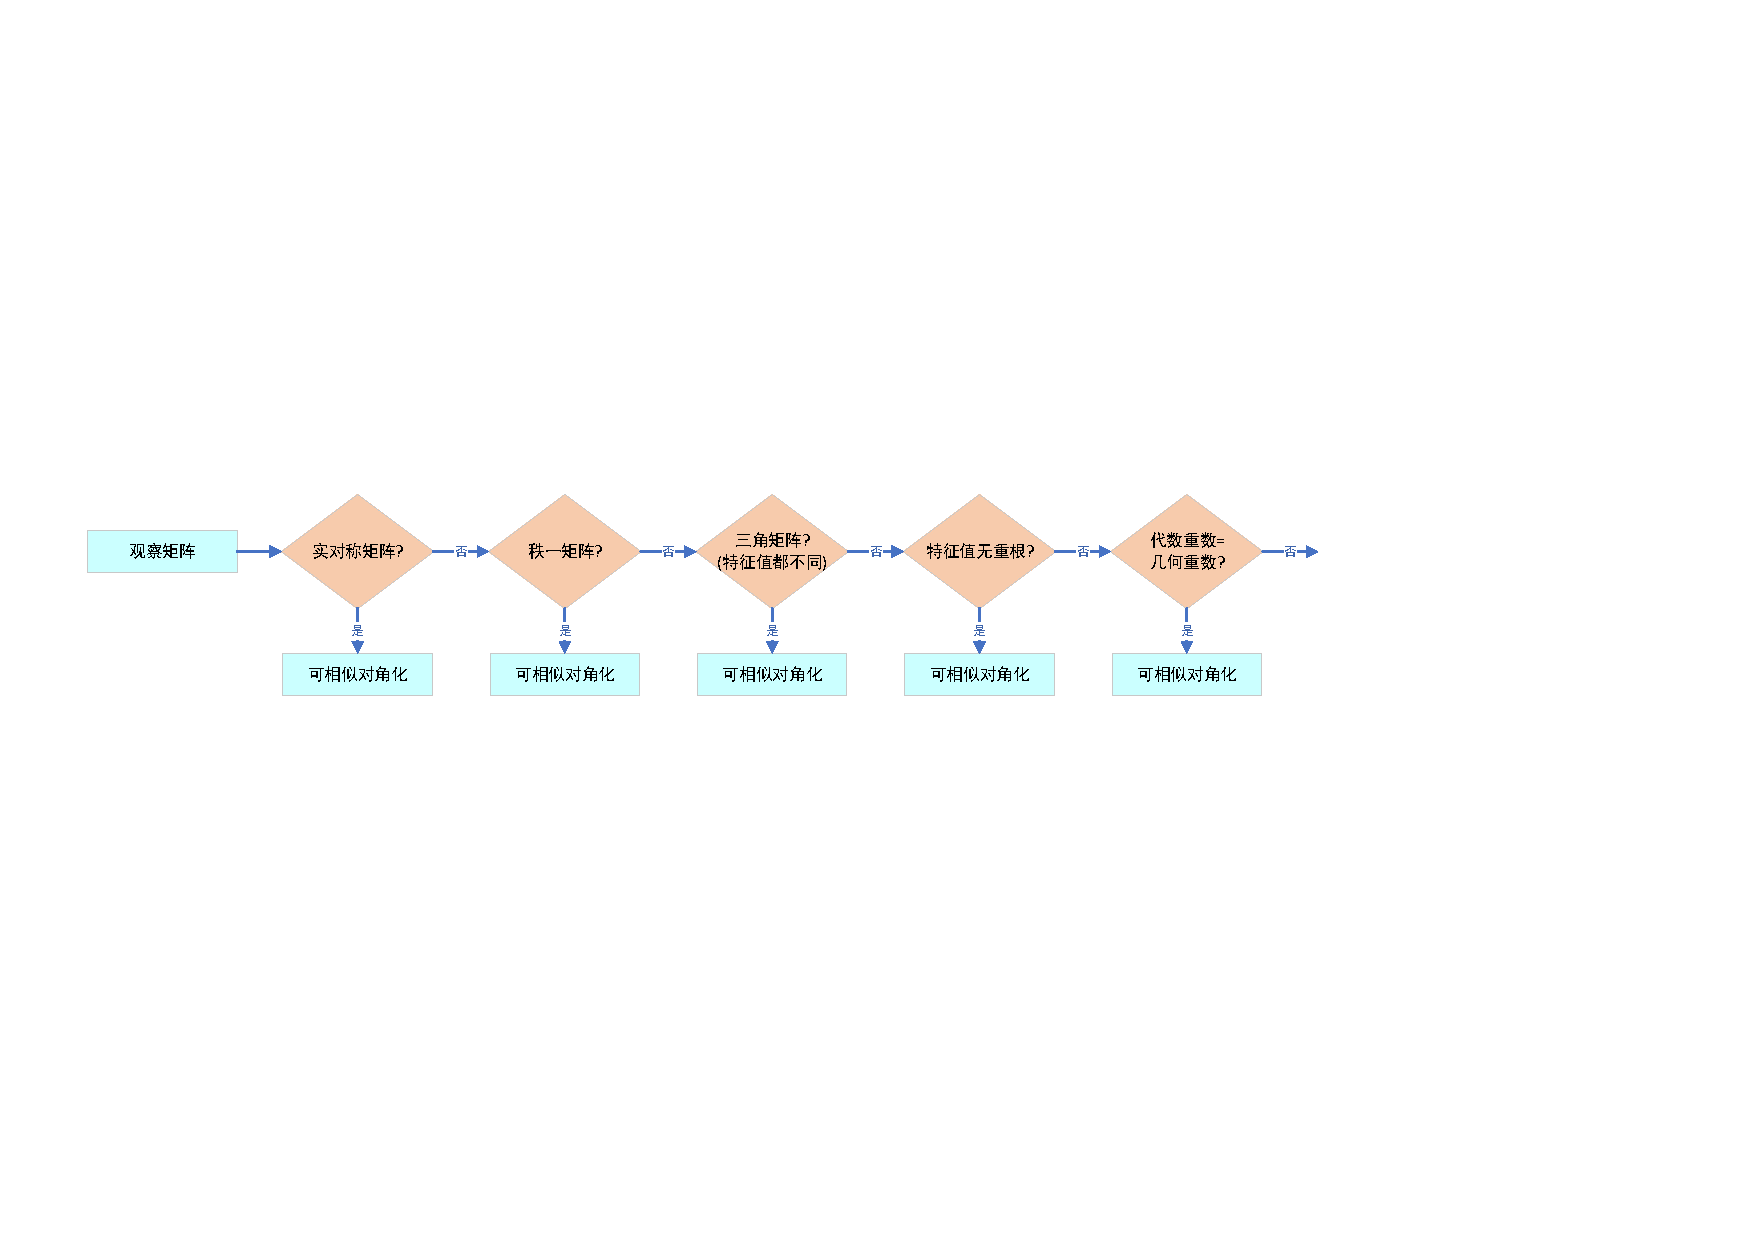
\includegraphics[scale=0.6]{figures/sdcjz.pdf}
%     \caption{}
%     \label{figure:sdcjz}
% \end{figure}

\begin{example}[2004 数一]
    设矩阵 $\vb*{A}=\mqty(1&2&-3\\-1&4&-3\\1&a&5)$ 的特征方程有一个二重根, 求 $a$ 的值, 并讨论 $\vb*{A}$ 是否可相似对角化.
\end{example}
\begin{solution}
    $|\lambda\vb*{E}-\vb*{A}|=\mqty|\lambda-1&-2&3\\1&\lambda-4&3\\-1&-a&\lambda-5|\xlongequal[r_2+r_3]{r_1-r_2}\mqty|\lambda-2&2-\lambda&0\\0&\lambda-4-a&\lambda-2\\-1&-a&\lambda-5|=(\lambda-2)\qty[(\lambda-5)(\lambda-4-a)+(\lambda-2)(1+a)]$,
    当 $\lambda=2$ 是方程的二重根时, 则有 $(2-5)(2-4-a)=0\Rightarrow a=-2$, 于是 $\vb*{A}=\mqty(1&2&-3\\-1&4&-3\\1&-2&5)$, 此时,
    $$\rank(2\vb*{E}-\vb*{A})=\rank\mqty(1&-2&3\\1&-2&3\\-1&2&-3)=\rank\mqty(0&0&0\\0&0&0\\-1&2&-3)=1=3-2$$
    因此可以相似对角化; 当 $2$ 不是方程的二重根时, $[(\lambda-5)(\lambda-4-a)+(\lambda-2)(1+a)]$ 为完全平方数, 解得 $a=-\dfrac{2}{3}$, 此时 $4$ 是该方程的二重根,
    于是 $\vb*{A}=\mqty(1&2&-3\\-1&4&-3\\1&-\dfrac{2}{3}&5)$, $\rank(4\vb*{E}-\vb*{A})\neq 1$, 于是 $a=-\dfrac{2}{3}$ 时, $\vb*{A}$ 不能相似对角化.
\end{solution}
